% \pdfoutput=1    % apparently this is needed at the beginning for arXiv to process it

% \documentclass[letterpaper, 10 pt, conference]{ieeeconf}
\documentclass[letterpaper, 10 pt, journal, twoside]{IEEEtran}


\IEEEoverridecommandlockouts                              % This command is only needed if 
                                                          % you want to use the \thanks command

% \overrideIEEEmargins                                      % Needed to meet printer requirements. Comment this for final RAL version, but keep it for final conference version.

% numbers option provides compact numerical references in the text. 
% \usepackage[numbers]{natbib}
\usepackage{multicol}
\usepackage[bookmarks=true]{hyperref}

% Various packages
\usepackage{float}
\usepackage{comment}
\usepackage{array}
\usepackage{graphicx}
\usepackage{booktabs}
\usepackage{multirow}

% Various math packages
\usepackage{amsmath}								
\usepackage{amssymb}
\usepackage{latexsym}
\usepackage{amsthm}
\usepackage{bm}
\usepackage{commath}
\usepackage{float}
\usepackage{units}

% packages for drawings
\usepackage{tikz}
% \usetikzlibrary{external}
% \tikzexternalize[prefix=tikz/] % activate!
\usetikzlibrary{arrows,shapes,trees,calc}
\usetikzlibrary{backgrounds}
\usepackage{pgfplots}
\pgfplotsset{compat=1.14}
\usepgfplotslibrary{polar}
\usepgfplotslibrary{patchplots}

% % reduce white space after captions
% \setlength{\textfloatsep}{10pt}

%% downsample images to make file smaller
%\usepackage{epstopdf}
%\epstopdfDeclareGraphicsRule{.pdf}{png}{.png}{convert #1 \OutputFile}
%\DeclareGraphicsExtensions{.png,.pdf}

% packages for 3d plotting with tikz
\usepackage{tikz-3dplot} %requires 3dplot.sty to be in same directory, or in your LaTeX installation
%\usepackage[active,tightpage]{preview}  %generates a tightly fitting border around the work
%\PreviewEnvironment{tikzpicture}
%\setlength\PreviewBorder{2mm}

% Commands for theorems
\newtheorem{definition}{Definition}[section]
\newtheorem{theorem}{Theorem}[section]
\newtheorem{assumption}{Assumption}[section]

% Definitions of custom colors
\definecolor{lightyellow}{RGB}{255,236,132}
\definecolor{lightgreen}{RGB}{161,239,10}
\definecolor{darkgreen}{RGB}{61,124,68}
\definecolor{lightblue}{RGB}{72,131,219}
\definecolor{darkblue}{RGB}{39,63,186}
\definecolor{plgreen}{RGB}{27,158,119}
\definecolor{plorange}{RGB}{217,95,2}
\definecolor{plpurple}{RGB}{117,112,179}
\definecolor{plpink}{RGB}{231,41,138}


% Editing tools
\usepackage{color}  % For Highlighting
\newcommand{\hilight}[1]{\colorbox{yellow}{#1}}
\newcommand{\David}[1]{\textcolor{red}{(#1)}}
\newcommand{\Ram}[1]{\textcolor{blue}{(#1)}}
\newcommand{\Dan}[1]{\textcolor{magenta}{(#1)}}
\newcommand{\Audrey}[1]{\textcolor{maroon}{(#1)}}

% Set macros to make certain things easier
\newcommand{\bmx}{\begin{bmatrix}}
\newcommand{\emx}{\end{bmatrix}}
\newcommand{\D}{\bar{\mathcal{D}}}

% Load and define stuff needed to add labels in the margins
\usepackage{marginnote}
% \makeatletter
% \let\oldmarginnote\marginnote
% \renewcommand*{\marginnote}[1]{%
%   \begingroup%
%   \ifodd\value{page}
%      \if@firstcolumn\reversemarginpar\fi
%   \else
%      \if@firstcolumn\else\reversemarginpar\fi
%   \fi
%   \oldmarginnote{#1}%
%   \endgroup%
% }
% \makeatother

% Set macro for labeling edits
\newcommand{\revcomment}[2]{\textcolor{red}{#2} \marginnote{\##1}} % Include reference commands
\renewcommand{\revcomment}[2]{#2}   % removes coloring of edited sections, i.e. makes doc look normal (comment this line out for highlighted edits)


\title{\LARGE \bf
Force Generation by Parallel Combinations of \\ Fiber-Reinforced Fluid-Driven Actuators
}


\author{Daniel Bruder$^{1}$, %<-this % stops a space
        Audrey Sedal$^{1}$, %
        Ram Vasudevan$^{1}$, %
        and C. David Remy$^{1}$%
\thanks{Manuscript received: February, 25, 2018; Revised May, 29, 2018; Accepted July, 9, 2018.}    % use only for final RAL version
\thanks{This paper was recommended for publication by Editor Yu Sun upon evaluation of the Associate Editor and Reviewers' comments.
*This material is supported by the Toyota Research Institute, and is based upon work supported by the National Science Foundation Graduate Research Fellowship Program under Grant No. 1256260 DGE. Any opinions, findings, and conclusions or recommendations expressed in this material are those of the author(s) and do not necessarily reflect the views of the National Science Foundation.}% <-this % stops a space
\thanks{$^{1}$ The authors are with the Mechanical Engineering Department at the 
        University of Michigan, Ann Arbor, MI 48109, USA
        {\tt\small \{bruderd, asedal, ramv, cdremy\}@umich.edu}}%
\thanks{Digital Object Identifier (DOI): see top of this page.}
% \thanks{This work has been submitted to the IEEE for possible publication. Copyright may be transferred without notice, after which this version may no longer be accessible.}   % for archive version only
}

\begin{document}

\maketitle
% \thispagestyle{empty}         % commented for final RAL version
% \pagestyle{empty}             % commented for final RAL version

% Paper headers (for final RAL submission)
\markboth{IEEE Robotics and Automation Letters. Preprint Version. Accepted July, 2018}
{Bruder \MakeLowercase{\textit{et al.}}: Force Generation by Parallel Combinations of Fluid-Driven Actuators}  % Use only for final RAL version

\begin{abstract}
\begin{abstract}
\label{sec:abstract}

%% 1. what is the problem 
Scientific applications that run on leadership computing facilities often face the challenge 
of being unable to fit leading science cases onto accelerator devices due to memory constraints 
(memory-bound applications).
%
% 2. what is your solution 
In this work, the authors studied one such US Department of Energy mission-critical condensed matter 
physics application, Dynamical Cluster Approximation (DCA++), and this paper discusses how device memory-bound challenges were successfully reduced  by proposing an effective 
``all-to-all'' communication method---a ring communication algorithm. 
%
This implementation takes advantage of acceleration on GPUs and remote direct memory access (RDMA) for fast data exchange between GPUs. 
%
\\Additionally, the ring algorithm was optimized with sub-ring communicators
and multi-threaded support to further reduce communication overhead and 
expose more concurrency, respectively.
%
% 3. What's the cherry-picked evaluation result you want to mention
The computation and communication were also analyzed 
by using the Autonomic Performance Environment for Exascale 
(APEX) profiling tool,  and this paper further discusses the 
performance trade-off for the ring algorithm implementation. 
%
The memory analysis on the ring algorithm shows that the allocation size for the authors' most 
memory-intensive data structure per GPU is now reduced to $1/p$ of the original size, where $p$ is the number of GPUs in the ring communicator.
%
The communication analysis suggests that 
the distributed Quantum Monte Carlo execution time grows linearly as sub-ring size increases, and the cost of messages passing through the network interface connector could be a limiting factor.


%
% \todoRed{Ronnie: Next sentence needs rewrite, too much information about Green's function that no one knows in the abstract; recommend generalizing.} \emph {However, DCA++ is currently facing memory-bound challenge as 
% a larger device array $G_t$ is limited by device memory size, where
% $G_t$ is a two-particle Green's function that allows condensed matter
% scientists to explore larger and more complex (higher fidelity)
% physics cases.}

\end{abstract}

\keywords{DCA++, Quantum Monte Carlo, GPU Remote Direct Memory Access, memory-bound issue, exascale machines}

\end{abstract}

% Keywords appear just beneath the abstract. Use only for final RAL version.
\begin{IEEEkeywords}
Soft Material Robotics, Hydraulic/Pneumatic Actuators, Force Control
\end{IEEEkeywords}

\IEEEpeerreviewmaketitle

% %!TEX ROOT = ../../centralized_vs_distributed.tex

%\subsection{Paper outline}\label{sec:outline}

\begin{table}
	\centering
	\caption{Theoretical tools (italic) and technical results (roman).}
	\label{tab:results}
	\footnotesize
	\begin{tabular}{|c|c|c|c|}
		\hline
		 & \textbf{Model} & \textbf{Stability} & \textbf{Variance} \\
		\hline
		\multirow{5}{*}{\shortstack{\textbf{Cont.} \\\textbf{time} \\\textbf{(CT)}}} & 
										\makecell{Single int. \\ \eqref{eq:cont-time-single-int-model},\eqref{eq:prop-control}} & 
										\makecell{\textit{Scalar SDDEs~\cite{KuchlerLangevinEqs}} \\ 
											Closed form~\eqref{eq:cont-time-single-int-variance-condition}} &
										\makecell{\textit{Scalar SDDEs~\cite{KuchlerLangevinEqs}} \\
											Closed form~\eqref{eq:cont-time-single-int-steady-state-variance}} \\
		\cline{2-4}
									& \makecell{Double int.\\ \eqref{eq:cont-time-double-int-model}--\eqref{eq:control-input-PD}} & 
									\makecell{\textit{Exponential} \\ \textit{polynomials~\cite{BAPTISTINI1997259}} \\ 
										\textit{SDDEs~\cite{datko1978procedure,wangBoundedness}} \\
										{Implicit}~\eqref{eq:cont-time-double-int-stability-condition}} & 
									\makecell{\textit{SDDEs~\cite{wangBoundedness}, time-}\\
										\textit{scale separation~\cite{khalil2002nonlinear}}\\
										{Integral form}~\eqref{eq:2nd-order-cont-ss-variance}\\
										Approximated~\eqref{eq:x-dynamics-1st-order-approximation}} \\
		\hline
		\multirow{4}{*}{\shortstack{\textbf{Disc.} \\ \textbf{time} \\\textbf{(DT)}}} &  
										\makecell{Single int. \\ \eqref{eq:disc-time-single-int-model},\eqref{eq:prop-control}} & 
										\makecell{\textit{Root locus~\cite{Westphal2001}}\\ 
											Closed form~\eqref{eq:disc-time-single-int-stability-condition}} &
										\makecell{\textit{Moment matching w/} \\
											\textit{Yule-Walker eqs.~\cite{yuleWalkerEqs}} \\
											{Recursive}~\eqref{eq:disc-time-single-int-moment-matching-eqs},\eqref{eq:disc-time-single-int-variance-explicit}} \\
		\cline{2-4}
									&  \makecell{Double int. \\ \eqref{eq:disc-time-double-int-model}} & 
									\makecell{\textit{Jury criterion~\cite{Jury}} \\ 
										{Closed form}~\eqref{eq:disc-time-double-int-characteristic-polinomial}} &
									\makecell{\textit{Moment matching w/} \\
										\textit{Yule-Walker eqs.~\cite{yuleWalkerEqs}} \\
										{Closed form}~\eqref{eq:disc-time-double-int-moment-matching-eqs}} \\
		\hline
	\end{tabular}
\end{table}

\myParagraph{\titlecap{Paper outline}}
In~\autoref{sec:setup} we describe models for communication and controller architecture
and formulate the minimum-variance control design problem.
\revision{While we first utilize ring topology to provide analytical insight
we also demonstrate that our framework can be extended to general undirected topologies; see~\autoref{sec:generic-topology}.}\linebreak
\revision{In Sections~\ref{sec:cont-time}--\ref{sec:cont-time-single-int-control-design}, we %solve the problem for continuous-time agent dynamics,
lay the ground for our main result.
In~\autoref{sec:cont-time}, 
we derive conditions for mean-square stability 
and compute the steady-state variance of continuous-time stochastically forced systems
using Stochastic Delay Differential Equations (SDDEs). 
In~\autoref{sec:cont-time-single-int-control-design},
we prove that the control design problem is convex} \review{and in 
\revision{\autoref{sec:numerical-results} we present} our main results:
by numerically computing the optimal controller gains,
we show that the closed-loop performance is optimized by sparse architectures.
Furthermore, 
we derive analytical expression~\eqref{eq:trade-off} for continuous-time single-integrator dynamics 
which demonstrates that the minimizer is in general nontrivial.}
To address wireless communication,
we study discrete-time systems in~\autoref{sec:disc-time}
and show that the fundamental behavior of the system does not change.
\autoref{tab:results} summarizes our technical results and the theoretical tools used throughout the paper.
\revision{Apart from classical control techniques such as the Jury stability criterion,
we also leverage more unconventional tools from mathematical literature,
such as exponential polynomials~\cite{BAPTISTINI1997259}.}
Concluding remarks are given in~\autoref{sec:conclusion}.

% Input sections here
\section{Introduction}  \label{sec:introduction}

\newcommand\inexpIntro[3]{#1?(#2,#3).}
\newcommand\rinexpIntro[3]{*#1?(#2,#3).}
\newcommand\outexpIntro[3]{#1!(#2,#3).}
\newcommand\outatomIntro[3]{#1!(#2,#3)}

We propose a fully automated method for proving termination of \(\pi\)-calculus processes.
Although there have been a lot of studies on termination analysis for the \(\pi\)-calculus
and related calculi~\cite{Deng06IC,Demangeon07,SangiorgiTermination,KobayashiHybrid,Yoshida04IC,DBLP:journals/jlp/DemangeonHS10,Venet98SAS}, most of them have been rather theoretical,
and there have been surprisingly little efforts in developing  fully automated termination
verification methods and tools based on them. To our knowledge,
Kobayashi's \typical{}~\cite{TyPiCal,KobayashiHybrid} is the only exception that
can prove termination of \(\pi\)-calculus processes (extended with natural numbers)
fully automatically, but its termination analysis is quite limited (see Section~\ref{sec:relatedwork}).

Our method is based on a reduction to termination analysis for sequential programs:
we translate a \(\pi\)-calculus process \(P\) to a sequential program \(S_P\), so that
if \(S_P\) is terminating, so is \(P\). The reduction allows us to use
powerful, mature methods and tools
for termination analysis of sequential programs~\cite{heizmann2016ultimate,freqterm,DBLP:conf/lics/PodelskiR04,Kuwahara2014Termination,DBLP:journals/cacm/CookPR11}.

The idea of the translation is to convert a chain of communications on replicated input
channels to a chain of recursive function calls of the target sequential program.
Let us consider the following Fibonacci process:
\begin{align*}
    & \rinexpIntro{\fib}{n}{r}
        \ifexp{n<2}{ \soutatom{r}{1} \\ &\quad}
                   { \nuexp{s_1} \nuexp{s_2} (\outatomIntro{\fib}{n-1}{s_1} \PAR \outatomIntro{\fib}{n-2}{s_2} \PAR \sinexp{s_1}{x}\sinexp{s_2}{y}\soutatom{r}{x+y}) \\}
    & \PAR \outatomIntro{\fib}{m}{r}
\end{align*}
Here, the process
$\rinexpIntro{\fib}{n}{r} \ldots$ is a function server that computes the \(n\)-th Fibonacci number
in parallel and returns the result to \(r\),
and $\outatom{\fib}{m}{r}$ sends a request for computing the \(m\)-th Fibonacci number;
those who are not familiar with the syntax of the \(\pi\)-calculus may wish to consult
Section~\ref{sec:targetlanguage} first.
To prove that the process above is terminating for any integer \(m\),
it suffices to show that there is no infinite chain of communications on $\fib$:
\[
    \fib(m,r) \to \fib(m_1,r_1) \to \fib(m_2,r_2) \to \cdots.
\]
We convert the process above to the following program:\footnote{The actual translation
  given later is a little more complex.}
\begin{verbatim}
 let rec fib(n) = if n<2 then () else (fib(n-1) [] fib(n-2)) in
 fib(m)
\end{verbatim}
Here, \texttt{[]} represents the non-deterministic choice.
Note that, although the calculation of Fibonacci numbers is not preserved,
for each chain of communications on \texttt{fib}, there is a corresponding
sequence of recursive calls:
\[
\mathtt{fib}(m) \to \mathtt{fib}(m_1) \to \mathtt{fib}(m_2) \to \cdots.
\]
Thus, the termination of the sequential program above implies the termination of
the original process.
As shown in the example above, (i) each communication on a replicated input channel
is converted to a function call, (ii) each communication on a non-replicated input
channel is just removed (or, in the actual translation, replaced by a call of
a trivial function defined by \(f(\seq{x})=(\,)\)), and (iii) parallel composition
is replaced by a non-deterministic choice.
We formalize the translation outlined above and prove its correctness.

The basic translation sketched above sometimes loses too much information.
For example, consider the following process:
\begin{align*}
    & \rinexpIntro{\pre}{n}{r} \soutatom{r}{n-1} \\
    & \PAR \rinexpIntro{f}{n}{r} \ifexp{n<0}{ \soutatom{r}{1} }
                                       { \nuexp{s} (\outatomIntro{\pre}{n}{s} \PAR \sinexp{s}{x}\outatomIntro{f}{x}{r}) } \\
    & \PAR \outatomIntro{f}{m}{r}
\end{align*}
The translation sketched above would yield:
\begin{verbatim}
  let pred(n) = n-1 in
  let rec f(n) = if n<0 then () else (pred(n) [] f(*)) in
  f(m)
\end{verbatim}
Here, \texttt{*} represents a non-deterministic integer: since we have removed
the input $\sinatom{s}{x}$, we do not have information about the value of \( x \).
As a result, the sequential program above is non-terminating, although the original
process is terminating.
To remedy this problem, we also refine the basic translation above by using a refinement
type system for the \(\pi\)-calculus. Using the refinement type system,
we can infer that the value of \(x\) in the original process is less than \(n\),
so that we can refine the definition of \texttt{f} to:
\begin{verbatim}
 let rec f(n) = ... else (pred(n) [] let x=* in assume(x<n);f(x))
\end{verbatim}
The target program is now terminating, from which
we can deduce that the original process is also terminating.
We have implemented an automated tool based on the refined translation above.

The contributions of this paper are summarized as follows.
\begin{itemize}
\item The formalization of the basic translation from the \(\pi\)-calculus
  (extended with integers) to sequential programs, and a proof of its correctness.
\item The formalization of a refined translation based on a refinement type system.
\item An implementation of the refined translation, including automated refinement type
  inference based on CHC solving, and experiments to evaluate the effectiveness of
  our method.
\end{itemize}

The rest of this paper is structured as follows.
Section~\ref{sec:targetlanguage} introduces the source and target languages
of our translation.
Section~\ref{sec:approach} 
formalizes the basic translation, and proves its correctness.
Section~\ref{sec:refinement} refines the basic translation by using a refinement type system.
Section~\ref{sec:implementation} reports an implementation and experiments.
Section~\ref{sec:relatedwork} discusses related work,
and Section~\ref{sec:conclusion} concludes the paper.

\section{Modeling}
\label{sec:singleActuator}
%
Our modeling approach for individual FREEs is based on the notion of a \emph{fluid Jacobian} $\bar{J}$, which maps the geometrical deformation of a soft actuator, or of a system of actuators, to a change in their volume. 
Under certain assumptions, the transpose of this Jacobian linearly maps the internal fluid pressure to the spatial forces that the actuator generates. 
One can  think of this fluid Jacobian as the soft and multi-dimensional equivalent of the cross section $A$ of a traditional pneumatic or hydraulic cylinder,
since this cross section similarly relates cylinder pressure to force, and piston movement to fluid displacement.


\subsection{Force Generation in a Single FREE}
%
The approach presented in this paper is enabled by a number of simplifying assumptions.
They are consistent with those made in prior work on the modeling and control of individual FREEs \cite{bishop2015design,bruder2017model}.
In particular, we assume that the fibers are inextensible and that they are uniformly  distributed  around  an elastomeric cavity  with negligible  wall thickness.
%The internal pressure in this cavity is uniform along its entire length.
Under these assumptions, a FREE can be modeled as a composition of an energy transforming element (the fibers) and an energy storing element (the compliance of the elastomer body). 
The generalized forces generated by each of these separate elements can be superimposed to characterize the net force $\vec{\tau}_{total}$ produced by the FREE:
\begin{align}
   \vec{\tau}_{\text{total}} &=  \vec{\tau} + \vec{\tau}_{\text{elast}}    \label{eq:netF}
\end{align}
where $\vec{\tau}$ and $\vec{\tau}_{\text{elast}}$ are the generalized forces and torques attributed to the fiber and elastomer, respectively.
In this work, we focus exclusively on the active general forces $\vec{\tau}$ that are generated by the fibers and that can be controlled by varying the pressure of the fluid.


The fluid Jacobian for such an actuator can be derived from the idea that the reinforcing fibers in a FREE create a kinematic constraint on the internal volume $V$ of the fluid cavity.
Without the reinforcing fibers, this cavity could expand freely, since it is made from soft material.
With the fibers, however, the volume is limited.
This limitation on volume depends on the mechanical parameters of the FREE (e.g., the relaxed fiber angle or fiber length) and on the current state of geometric deformation of the FREE.
This geometric state can be represented by a generalized vector of spatial deformations $\vec{q}$:  $V = V\left(\vec{q}\right)$.


The derivative of this volume yields an expression $\dot{V}$ for the volumetric flow into the actuator:
\begin{align}
    \dot{V} (\vec{q}, \dot{\vec{q}}) &= \frac{\partial V}{\partial t} = \frac{\partial V}{\partial \vec{q}} \frac{\partial \vec{q}}{\partial t } = \bar{J}_q (\vec{q}) \dot{\vec{q}},  \label{eq:Vdot_wJ}
\end{align}
where the fluid Jacobian is defined as $\bar{J}_{q}= \frac{\partial V}{\partial \vec{q}}$ with respect to the deformation $\vec{q}$. 


It is important to note that $\vec{\tau}$ and $\dot{\vec{q}}$ live in dual spaces. 
That is, forces in $\vec{\tau}$ correspond to linear motion in $\dot{\vec{q}}$, and moments in $\vec{\tau}$ correspond to angular motion in $\dot{\vec{q}}$.
In the most general case, these are 6-dimensional vectors with three translations and three rotations.
In this case, $\bar{J}_q$ is a $1 \times 6$ matrix.


Energy conservation dictates that the mechanical power generated by the fibers must equal the fluid power that goes into the FREE:
\begin{align}
    P_{\text{mech}} = P_{\text{fluid}} = \dot{\vec{q}}^{\,T} \vec{\tau} &= \dot{V} p, 
    \label{eq:Pequiv}
\end{align}
%
where $p>0$ is the pressure of the fluid inside the FREE.
Substituting \eqref{eq:Vdot_wJ} into \eqref{eq:Pequiv}, we arrive at a linear expression that yields the forces produced by the FREE fibers as a function of deformation state and fluid pressure: 
\begin{align}
    \vec{\tau} (\vec{q}, p) &= \bar{J}_q^T (\vec{q}) p       \label{eq:fiberF}
\end{align}
The fluid Jacobian thus describes the generalized direction in which a FREE can produce forces and torques.
Since the input pressure $p$ needs to be strictly positive to avoid collapsing of the fluid cavity, forces can only be produced in the positive direction defined by $\bar{J}_q$.


\subsection{The Fluid Jacobian of a Cylindrical FREE}
The theoretical modeling approach outlined above can be applied independently of the exact geometry of a FREE and can even be extended to other classes of soft actuators.
However, to make the computation of the fluid Jacobian tractable, we rely on another common assumption for FREES: that they maintain the geometry of an ideal cylinder \cite{bishop2015design}.
This neglects the tapering of the actuator towards the end-caps and any potential bending along its main axis.

\begin{figure}
    \centering
    \begin{tikzpicture}
        \node (FREEstate) at (0,0)
            {\includegraphics[width=0.75\linewidth]{figures/FREEstate_noLabels3.pdf}};
        \node[right] (a) at ($ (FREEstate.east) !0.5! (FREEstate.north east) $) {(a)};
        \node[right] (b) at ($ (FREEstate.east) !0.5! (FREEstate.south east) $) {(b)};
    \end{tikzpicture}
    \caption{Geometric parameters of an ideal cylindrical FREE in (a) the relaxed configuration where $\vec{q}=0$ (top), and (b) a deformed configuration where ${\vec{q}=\lbrack \Delta l \hspace{2pt} , \hspace{2pt} \Delta \phi \rbrack^T}$ (bottom).}
    \label{fig:FREEparams}
\end{figure}

An ideal cylindrical FREE in its relaxed configuration (i.e. when gauge fluid pressure is zero and no external loads are applied) can be described by a set of three parameters, $L$, $R$, and $\Gamma$, where $L$ represents the relaxed length of the FREE, $R$ represents the radius, and $\Gamma$ the fiber angle (Fig.~\ref{fig:FREEparams}). 
For notational convenience, we define two other quantities from these parameters:
\begin{align}
	B &= \left| \frac{L}{\cos{\Gamma}} \right| \\
	N &= - \frac{L}{2 \pi R} \tan{\Gamma}
\end{align}
where $B$ is the length of one of the FREE fibers, and $N$ is the total number of revolutions the fiber makes around the FREE in the relaxed configuration. 

\revcomment{2.4}{The assumption that a FREE is cylindrical with inextensible fiber-reinforcements implies that changes in its radius, length, and twist are coupled 
% via the right triangle relationship shown in Fig. \ref{fig:fiber}
. Therefore, its geometrical deformation can be fully defined in terms of just two parameters, a change in its length $\Delta l$ and a twist about its main axis $\Delta \phi$.}
These two values constitute the vector of generalized deformations $\vec{q} = \left[ \Delta l, \Delta \phi \right]^T$.
Consequently the generalized torque vector $\vec{\tau} = \left[ F, M \right]^T$ describes a force along the main axis, $F$, and a torsional moment about that axis, $M$.

From this, the length and radius of the deformed FREE can be computed according to:
\begin{align}
    l &= L + \Delta l \label{eq:l} \\
	r &= \frac{B}{\abs{2 \pi N + \Delta \phi}} \sqrt{1 - \left( \frac{L+\Delta l}{B} \right)^2}, \label{eq:r}
\end{align}
and we can express the volume as
\begin{align}
	V(\vec{q}) &= \pi r^2 l \notag \\ 
	&= \frac{\pi (L+\Delta l) (B^2 - (L+\Delta l)^2)}{(2 \pi N + \Delta \phi)^2}  \label{eq:V}.
\end{align}

With this, the fluid Jacobian evaluates to:
\begin{align}
    \bar{J}_q (\vec{q})
    &= \begin{bmatrix} 
		        \frac{\pi \left( B^2 - 3(L + \Delta l)^2 \right)}{(2 \pi N + \Delta \phi)^2} & \frac{2 \pi (L+\Delta l) \left( (L+\Delta l)^2 - B^2 \right)}{(2 \pi N + \Delta \phi)^3}
		\end{bmatrix}.    \label{eq:Jv}
\end{align}


% % THIS FIGURE WILL BE REMOVED FOR SPACE IF NEEDED, BUT I WANT TO KEEP IT IF POSSIBLE 
% \begin{figure}
%     \centering
%     \begin{tikzpicture}
%         \node (fiber) at (0,0)
%             {\includegraphics[width=0.85\linewidth]{figures/fiber_noLabels2.png}};
%         \node[below] (a) at ($ (fiber.south west) !0.08! (fiber.south east) $) {(a)};
%         \node[below] (b) at ($ (fiber.south west) !0.32! (fiber.south east) $) {(b)};
%         \node[below] (c) at ($ (fiber.south west) !0.75! (fiber.south east) $) {(c)};
%     \end{tikzpicture}
%     \caption{(a) A FREE contains many parallel fibers, all part of the same fiber family. (b) One isolated fiber forms a helical constraint. (c) The FREE radius $r$, twist $\Delta \phi$, and length change $\Delta l$ are geometrically related via the right triangle formed by unwinding a fiber and laying it flat.}
%     \label{fig:fiber}
% \end{figure}





\subsection{Parallel Combinations of FREEs}
\label{sec:parallelActuators}
We can extend the concept of a fluid Jacobian to systems with multiple actuators that are mounted in parallel.
FREEs that are mounted in parallel each have one end attached to a common ground and the other rigidly attached to an end effector.
The position and orientation of this end effector is given by a deformation vector $\vec{x}$, and we assume that an inverse kinematics function allows the computation of the state $\vec{q}_i \left(\vec{x}\right)$ for each individual FREE.
To express forces and torques in a common reference frame, we define a body-fixed reference point and coordinate system that are attached to the end effector (Fig.~\ref{fig:dp_defined}). 
Expressed in these coordinates, a position vector ${\vec{d}_i = \begin{bmatrix} d_i^{\hat{x}_e} & d_i^{\hat{y}_e} & d_i^{\hat{z}_e} \end{bmatrix}^T}$ defines the point where the $i$th FREE is attached, and a unit vector ${\hat{a}_i = \begin{bmatrix} a_i^{\hat{x}_e} & a_i^{\hat{y}_e} & a_i^{\hat{z}_e} \end{bmatrix}^T}$, expresses the direction of the associated FREE axis.

Let $\vec{f}_i$ be the vector of general forces exerted by the $i$th FREE and expressed in end effector coordinates:
\begin{align}
    \vec{f}_i = \bmx F^{\hat{x}_e}_i & F^{\hat{y}_e}_i & F^{\hat{z}_e}_i & M^{\hat{x}_e}_i & M^{\hat{y}_e}_i & M^{\hat{z}_e}_i \emx^T,
\end{align}
where $F^{\hat{x}_e}_i$ is the component of force along the $x$-axis of the end effector frame and $M^{\hat{x}_e}_i$ is the moment about the $x$-axis of that frame.
The components of this vector can be computed from the axial force $F_i$ and twisting torque $M_i$ of the $i$th FREE as:
\begin{align}
    \bmx F^{\hat{x}_e}_i & F^{\hat{y}_e}_i & F^{\hat{z}_e}_i \emx^T &= \hat{a}_i F_i ,   \label{eq:Df}
\end{align}
and
\begin{align}
    \bmx M^{\hat{x}_e}_i & M^{\hat{y}_e}_i & M^{\hat{z}_e}_i \emx^T &= \lfloor \vec{d}_i \times \rfloor \hat{a}_i F_i + \hat{a}_i M_i,    \label{eq:Dm}
\end{align}
where $\lfloor \vec{d}_i \times \rfloor$ is the matrix notation for the cross-product with $\vec{d}_i$:
\begin{align}
    \lfloor \vec{d}_i \times \rfloor &= \begin{bmatrix} 0 & -d_i^{\hat{z}_e} & d_i^{\hat{y}_e} \\ d_i^{\hat{z}_e} & 0 & -d_i^{\hat{x}_e} \\ -d_i^{\hat{y}_e} & d_i^{\hat{x}_e} & 0 \end{bmatrix}. 
\end{align}
Combining \eqref{eq:Df} and \eqref{eq:Dm} into a single transformation yields:
\begin{align}
    \vec{f}_i &= \bar{\mathcal{D}}_i \vec{\tau}_i,  \label{eq:zetai}
\end{align}
where $\mathcal{D}_{i}$ is the $6 \times 2$ matrix:
\begin{align}
    \bar{\mathcal{D}}_i &= \begin{bmatrix}
                    \begin{bmatrix} \hat{a}_i & \vec{0}_{3\times1} \end{bmatrix} \vspace{5pt} \\ 
                    \begin{bmatrix} \lfloor \vec{d}_i \times \rfloor \hat{a}_i & \vec{0}_{3\times1} \end{bmatrix} + \begin{bmatrix} \vec{0}_{3\times1} & \hat{a}_i \end{bmatrix}
                    \end{bmatrix}.   \label{eq:D}
\end{align}


\begin{figure}
    \centering
    \begin{tikzpicture}
        \node (diagram) at (0,0)
            {\includegraphics[width=1.0\linewidth]{figures/dp_defined-revised-v2.pdf}};
        \node[below] (a) at ($ (diagram.south west) !0.22! (diagram.south east) $) {(a)};
        \node[below] (b) at ($ (diagram.south west) !0.65! (diagram.south east) $) {(b)};
    \end{tikzpicture}
%    (a) An arbitrary combination of 3 FREEs connected to a common end effector. (b) A zoomed in view of the end effector with its local coordinate frame shown.}
    \caption{\revcomment{2.7}{(a) When multiple FREEs are attached in parallel to the same end effector, shown on the left, we must consider their relative positions and orientations. (b) This is determined by the vector $\vec{d}_i$ of the displacement of the attachment point of a FREE relative to the origin of the end effector frame, and by the unit vector $\hat{a}_i$ that is aligned with the FREE axis at the attachment point, shown in the zoomed-in view on the right.}}
    \label{fig:dp_defined}
\end{figure}


Since the actuators are mounted in parallel, the total force $\vec{f}$ is the sum of the individual forces of all $n$ FREEs connected to the end effector: 
\begin{align}
    \vec{f}(\vec{q}, \vec{p}) &= \sum_{i=1}^n \vec{f}_{i} = \sum_{i=1}^n \bar{\mathcal{D}}_i \bar{J}^T_{q, i} (\vec{q}_i) p_i = \sum_{i=1}^n \bar{J}^T_{x, i} (\vec{x}) p_i,
    \label{eq:zeta}
\end{align}
where $\bar{J}_{x, i} = \bar{J}_{q, i} \bar{\mathcal{D}}^T_i$ is the fluid Jacobian of an individual FREE expressed in end effector coordinates and the vector $\vec{p}$ contains the internal pressure values of all FREEs.

This can be written compactly in matrix notation as 
\begin{align}
    \vec{f} (\vec{x}, \vec{p}) &= \bar{J}^T_x (\vec{x}) \vec{p}, \label{DAVIDreallyLIKESthisEQUATION}
\end{align}
with the overall fluid Jacobian $\bar{J}_x$:
\begin{align}
    \bar{J}_x &= \bmx \bar{J}^T_{x, 1} & \bar{J}^T_{x, 2} & \cdots & \bar{J}^T_{x, n} \emx^T
\end{align}

\subsection{The Force Zonotope}
Equation \eqref{DAVIDreallyLIKESthisEQUATION} shows that the force capability of the parallel combination of multiple FREEs is a linear function of the pressures in the individual actuators.
Since the fluid Jacobian $\bar{J}_{x}$ depends on the end effector state $\vec{x}$, the ability of such a system to generate forces at the end effector will vary based on its displacement.
For some values of $\vec{x}$ it may be possible to generate spacial forces in multiple directions, while for others the span of possible forces may by narrower. 
The \emph{force zonotope} of a parallel combination of FREEs, similar to the force ellipsoid of rigid manipulators, 
% \cite{spong2008robot}
describes the set of forces that can be generated at the end effector with a bounded set of input pressures.

\begin{definition}[Force Zonotope]
    For a parallel combination of $n$ FREEs, the force zonotope is the set of active general 
%    torques and
    forces that can be generated in a specific end effector state, $\vec{x}$,
    \begin{align}
        \mathcal{Z}(\vec{x}) &= \left\{\bar{J}^T_x (\vec{x}) \vec{p} \, : \, p_i \in [0,p_i^\text{max}] \right\}     \label{eq:zonotope}
    \end{align}
    where $p_i^{\text{max}}$ is the maximum pressure allowed for the $i^{th}$ FREE.
\end{definition}

Note that the \emph{force zonotope} is the convex hull of all spacial forces generated when $p_i \in \{0, p_i^{\text{max}}\}$.
This makes it viable to compute using a convex hull algorithm. By calculating the zonotope over a range of states, it can be used to verify that a given parallel FREE design is capable of generating the desired forces over the range of its workspace. 
%In this way, the \emph{force zonotope} provides insight into how to utilize FREEs as actuators for robotic systems.


To illustrate the design utility of the force zonotope, consider the parallel combination of FREEs shown in Figure~\ref{fig:zntpConstructed}.
Here, pairs of FREEs with opposite chirality are connected to the two sides of an end effector.
This end effector is constrained to slide and rotate exclusively along and about its $z$-axis.
Since the motion of the end-effector is two-dimensional, we would like to achieve controllable forces within these two dimensions; that is, have control authority over $F^{\vec{z}_e}$ and $M^{\vec{z}_e}$.
When constructing the zonotope one FREE at time (Figure~\ref{fig:zntpConstructed}a-d), one can observe how all four FREEs are needed to achieve this control authority.
In particular, it becomes evident that to achieve full control in $n$ dimensions, at least $n+1$ individual FREEs are required in an antagonistic configuration.
The additional FREE is needed since these soft actuators cannot be driven with negative pressure and can hence not produce bidirectional forces.
One can also observe that if the FREEs are chosen or arranged poorly such that the directions in $\bar{J}_{x}$ do not cover the space of desired forces (such as in Fig.~\ref{fig:zntpConstructed}c), this minimum number of actuators might not be sufficient.

\begin{figure}
    \centering

\includegraphics[width=0.85\linewidth]{figures/zntpExampleRig3.pdf}

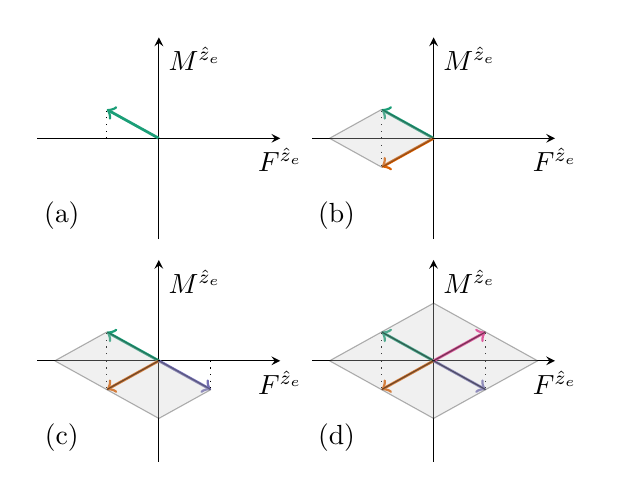
\begin{tikzpicture}
\def\scl{0.45} % define scale variable for plots

% PRACTICE PLOT
\matrix [row sep=0.25cm, column sep=0cm, style={align=center}] (my matrix) at (0,0)
{

\begin{axis}[
    view={90}{0},
    axis lines=center,
    % axis equal image,
    xlabel={$M^{\hat{x}_e}$},
    ylabel={$F^{\hat{z}_e}$},
    zlabel={$M^{\hat{z}_e}$},
    ymin=-7, ymax=7, ytick={0}, %ylabel near ticks,
    xmin=-5, xmax=10, xtick={0}, %xticklabel=$\pgfmathprintnumber{\tick}^\circ$, xlabel near ticks, 
    zmin=-7, zmax=7, ztick={0}, %z dir=reverse,
    xlabel style={anchor=north}, ylabel style={anchor=north},
    scale=\scl,
    anchor=center,
    name=plot1,
    ]
    \def\pa{(-2,-3,2)}
    \def\pb{(2,-3,-2)}
    \def\pc{(2,3,-2)}
    \def\pd{(-2,3,2)}
    \addplot3[->, line width=1pt, plgreen] coordinates {(0,0,0) \pa};
%    \addplot3[->, line width=1pt, plorange] coordinates {(0,0,0) \pb};
%    \addplot3[->, line width=1pt, plpurple] coordinates {(0,0,0) \pc};
%    \addplot3[->, line width=1pt, plpink] coordinates {(0,0,0) \pd};
    % connector lines for perspective
    \addplot3[dotted] coordinates {(0,0,0) (-2,-3,0)};
    \addplot3[dotted] coordinates {(-2,-3,0) \pa}; 
%    \addplot3[dotted] coordinates {(0,0,0) (2,-3,0)};
%    \addplot3[dotted] coordinates {(2,-3,0) \pb};
%    \addplot3[dotted] coordinates {(0,0,0) (2,3,0)};
%    \addplot3[dotted] coordinates {(2,3,0) \pc};
%    \addplot3[dotted] coordinates {(0,0,0) (-2,3,0)};
%    \addplot3[dotted] coordinates {(-2,3,0) \pd};
    % faces of shape
%    \addplot3[patch, opacity=0.3, fill=black!20, faceted color=black, patch type=rectangle] 
%        coordinates {
%                    (0,0,0) \pa (0,-6,0) \pb
%                    (0,0,0) \pb (4,0,-4) \pc
%                    (0,0,0) \pc (0,6,0) \pd
%                    (0,0,0) \pd (-4,0,4) \pa
%                    };
\end{axis};

&

\begin{axis}[
    view={90}{0},
    axis lines=center,
    % axis equal image,
    xlabel={$M^{\hat{x}_e}$},
    ylabel={$F^{\hat{z}_e}$},
    zlabel={$M^{\hat{z}_e}$},
    ymin=-7, ymax=7, ytick={0}, %ylabel near ticks,
    xmin=-5, xmax=10, xtick={0}, %xticklabel=$\pgfmathprintnumber{\tick}^\circ$, xlabel near ticks, 
    zmin=-7, zmax=7, ztick={0}, %z dir=reverse,
    xlabel style={anchor=north}, ylabel style={anchor=north},
    scale=\scl,
    anchor=center,
    name=plot2,
    ]
    \def\pa{(-2,-3,2)}
    \def\pb{(2,-3,-2)}
    \def\pc{(2,3,-2)}
    \def\pd{(-2,3,2)}
    \addplot3[->, line width=1pt, plgreen] coordinates {(0,0,0) \pa};
    \addplot3[->, line width=1pt, plorange] coordinates {(0,0,0) \pb};
%    \addplot3[->, line width=1pt, plpurple] coordinates {(0,0,0) \pc};
%    \addplot3[->, line width=1pt, plpink] coordinates {(0,0,0) \pd};
    % connector lines for perspective
    \addplot3[dotted] coordinates {(0,0,0) (-2,-3,0)};
    \addplot3[dotted] coordinates {(-2,-3,0) \pa}; 
    \addplot3[dotted] coordinates {(0,0,0) (2,-3,0)};
    \addplot3[dotted] coordinates {(2,-3,0) \pb};
%    \addplot3[dotted] coordinates {(0,0,0) (2,3,0)};
%    \addplot3[dotted] coordinates {(2,3,0) \pc};
%    \addplot3[dotted] coordinates {(0,0,0) (-2,3,0)};
%    \addplot3[dotted] coordinates {(-2,3,0) \pd};
    % faces of shape
    \addplot3[patch, opacity=0.3, fill=black!20, faceted color=black, patch type=rectangle] 
        coordinates {
                    (0,0,0) \pa (0,-6,0) \pb
%                    (0,0,0) \pb (4,0,-4) \pc
%                    (0,0,0) \pc (0,6,0) \pd
%                    (0,0,0) \pd (-4,0,4) \pa
                    };
\end{axis};


\\

\begin{axis}[
    view={90}{0},
    axis lines=center,
    % axis equal image,
    xlabel={$M^{\hat{x}_e}$},
    ylabel={$F^{\hat{z}_e}$},
    zlabel={$M^{\hat{z}_e}$},
    ymin=-7, ymax=7, ytick={0}, %ylabel near ticks,
    xmin=-5, xmax=10, xtick={0}, %xticklabel=$\pgfmathprintnumber{\tick}^\circ$, xlabel near ticks, 
    zmin=-7, zmax=7, ztick={0}, %z dir=reverse,
    xlabel style={anchor=north}, ylabel style={anchor=north},
    scale=\scl,
    anchor=center,
    name=plot3,
    ]
    \def\pa{(-2,-3,2)}
    \def\pb{(2,-3,-2)}
    \def\pc{(2,3,-2)}
    \def\pd{(-2,3,2)}
    \addplot3[->, line width=1pt, plgreen] coordinates {(0,0,0) \pa};
    \addplot3[->, line width=1pt, plorange] coordinates {(0,0,0) \pb};
    \addplot3[->, line width=1pt, plpurple] coordinates {(0,0,0) \pc};
%    \addplot3[->, line width=1pt, plpink] coordinates {(0,0,0) \pd};
    % connector lines for perspective
    \addplot3[dotted] coordinates {(0,0,0) (-2,-3,0)};
    \addplot3[dotted] coordinates {(-2,-3,0) \pa}; 
    \addplot3[dotted] coordinates {(0,0,0) (2,-3,0)};
    \addplot3[dotted] coordinates {(2,-3,0) \pb};
    \addplot3[dotted] coordinates {(0,0,0) (2,3,0)};
    \addplot3[dotted] coordinates {(2,3,0) \pc};
%    \addplot3[dotted] coordinates {(0,0,0) (-2,3,0)};
%    \addplot3[dotted] coordinates {(-2,3,0) \pd};
    % faces of shape
    \addplot3[patch, opacity=0.3, fill=black!20, faceted color=black, patch type=rectangle] 
        coordinates {
                    (0,0,0) \pa (0,-6,0) \pb
                    (0,0,0) \pb (4,0,-4) \pc
%                    (0,0,0) \pc (0,6,0) \pd
%                    (0,0,0) \pd (-4,0,4) \pa
                    };
\end{axis};

&

\begin{axis}[
    view={90}{0},
    axis lines=center,
    % axis equal image,
    xlabel={$M^{\hat{x}_e}$},
    ylabel={$F^{\hat{z}_e}$},
    zlabel={$M^{\hat{z}_e}$},
    ymin=-7, ymax=7, ytick={0}, %ylabel near ticks,
    xmin=-5, xmax=10, xtick={0}, %xticklabel=$\pgfmathprintnumber{\tick}^\circ$, xlabel near ticks, 
    zmin=-7, zmax=7, ztick={0}, %z dir=reverse,
    xlabel style={anchor=north}, ylabel style={anchor=north},
    scale=\scl,
    anchor=center,
    name=plot4,
    ]
    \def\pa{(-2,-3,2)}
    \def\pb{(2,-3,-2)}
    \def\pc{(2,3,-2)}
    \def\pd{(-2,3,2)}
    \addplot3[->, line width=1pt, plgreen] coordinates {(0,0,0) \pa};
    \addplot3[->, line width=1pt, plorange] coordinates {(0,0,0) \pb};
    \addplot3[->, line width=1pt, plpurple] coordinates {(0,0,0) \pc};
    \addplot3[->, line width=1pt, plpink] coordinates {(0,0,0) \pd};
    % connector lines for perspective
    \addplot3[dotted] coordinates {(0,0,0) (-2,-3,0)};
    \addplot3[dotted] coordinates {(-2,-3,0) \pa}; 
    \addplot3[dotted] coordinates {(0,0,0) (2,-3,0)};
    \addplot3[dotted] coordinates {(2,-3,0) \pb};
    \addplot3[dotted] coordinates {(0,0,0) (2,3,0)};
    \addplot3[dotted] coordinates {(2,3,0) \pc};
    \addplot3[dotted] coordinates {(0,0,0) (-2,3,0)};
    \addplot3[dotted] coordinates {(-2,3,0) \pd};
    % faces of shape
    \addplot3[patch, opacity=0.3, fill=black!20, faceted color=black, patch type=rectangle] 
        coordinates {
                    (0,0,0) \pa (0,-6,0) \pb
                    (0,0,0) \pb (4,0,-4) \pc
                    (0,0,0) \pc (0,6,0) \pd
                    (0,0,0) \pd (-4,0,4) \pa
                    };
\end{axis};

\\
};

\node[above] (a2) at ($ (plot1.south west) !0.1! (plot1.south east) $) {(a)};
\node[above] (b2) at ($ (plot2.south west) !0.1! (plot2.south east) $) {(b)};
\node[above] (c2) at ($ (plot3.south west) !0.1! (plot3.south east) $) {(c)};
\node[above] (d2) at ($ (plot4.south west) !0.1! (plot4.south east) $) {(d)};

\end{tikzpicture}

    \caption{An end effector is driven by the parallel combination of two pairs of FREEs with opposing chirality.
    The zonotope (grey areas) is the range of forces that can be produced by applying strictly positive pressure to the individual FREEs.
    It is spanned by the individual force vectors that each FREE produces at maximal pressure (plotted here in the color corresponding to the FREE's appearance in the diagram above).
    By constructing the zonotope for (a) one FREE, (b) two FREEs, (c) three FREEs, (d) four FREEs in parallel, one can observe that all four actuators are needed to gain full control authority over forces along and torques about the $z$-axis.
    In this poorly designed system (with fiber angles and attachments points as shown in the top diagram), the theoretical minimum of 3 actuators is not sufficient to achieve full control authority.}
    \label{fig:zntpConstructed}
\end{figure}






















\newcommand{\twomoons}{{\tt Twomoons}}
\newcommand{\gauss}{{\tt Gauss}}
\newcommand{\sculpture}{{\tt Sculpture}}
\newcommand{\baseline}{{\tt Baseline}}
\newcommand{\MM}{{\tt MsgPassing}}
\newcommand{\blackboard}{{\tt Blackboard}}
\newcommand{\ncut}{\text{ncut}}
\newcommand{\chensays}[2][]{\textcolor{blue} {\textsc{Jiecao #1:} \emph{#2}}}

\section{Experiments}
In this section we present experimental results for  graph clustering in the message passing and blackboard models. We will compare the following three algorithms. (1) \baseline: each site sends all the data to the coordinator directly; (2) \MM: our algorithm in the message passing model (Section~\ref{sec:gcmessage}); (3) 
\blackboard: our algorithm in  the blackboard model (Section~\ref{sec:bb}).


%Since both of our algorithms are crucially based on the use of spectral scarification, our main focus in the experiments is to investigate to what extend the quality of the spectral clustering algorithms will be affected by using spectral sparsification, the saving of communication costs by using spectral sparsificaion, ...
%
%
%The goal of this experiment is not to demonstrate the effectiveness of the spectral clustering algorithm. We mainly want to investigate the following, 
%\begin{itemize}
%\item to what extend the quality of clustered results will be affected by using spectral sparsification.
%\item saving of communication costs by using spectral sparsifier.
%\item the affect of constants in algorithms of the message passing/blackboard model.
%\end{itemize}
%
%
%\subsection{The Setup}
%\paragraph{Reference Algorithms}
%We compare different algorithms in our experiment.

%Note that we can also run \MM~ in the blackboard model.

Besides giving the visualized results of these algorithms on various datasets, we also measure the qualities of the results via the {\em normalized cut}, defined as 
\[
\ncut(A_1, \ldots, A_{k}) = \frac{1}{2}\sum_{i\in[k]}\frac{w(A_i, V\backslash A_i)}{\vol(A_i)},
\]
 which is a standard objective function to be minimized for spectral clustering algorithms. 
%We will compare the communication costs of these algorithms in different settings.

%We also compare the total communication costs of different algorithms/models. As the unit does not matter in our case, we normalize all communication costs by the cost of \baseline.  Whenever possible, we will visualize the clustered results.

We implemented the algorithms using multiple languages, including Matlab, Python and C++. Our experiments were conducted on an IBM NeXtScale nx360 M4 server, which is equipped with 2 Intel Xeon E5-2652 v2 8-core processors, 32GB RAM and 250GB local storage.


\subsection{Datasets.}
We test the algorithms in the following real and synthetic datasets, which is visualized in \figref{visualization}.


\begin{figure}[h]
     \centering
     \subfigure[\twomoons]{\includegraphics[width=0.23\textwidth]{twomoons-14000-original.png}\label{fig:twomoons}}
     ~~
     \subfigure[\gauss]{\includegraphics[width=0.23\textwidth]{gauss-10000-original.png}\label{fig:gauss}}
     ~~
     \subfigure[\sculpture]{\includegraphics[width=0.13\textwidth,height=0.16\textwidth]{sculpture-11680-original.jpg}\label{fig:sculpture}}
     \caption{Visualization of the datasets for our experiments.}
     \label{fig:visualization}
\end{figure}



\vspace{-1mm}
\begin{itemize}
\item \twomoons : this dataset contains $n=14,000$ coordinates in $\mathbb{R}^2$. We consider each point to be a vertex. For any two vertices $u, v$, we add an edge with weight $w(u,v) = \exp\{-\|u-v\|_2^2/\sigma^2\}$ with $\sigma = 0.1$ when one vertex is among the $7000$-nearest points of the other.  This construction results in a graph with about $110,000,000$ edges.

\item  \gauss : this dataset contains $n = 10,000$ points in $\mathbb{R}^2$. There are $4$ clusters in this dataset, each generated using a Gaussian distribution. We construct a complete graph as the similarity graph.  For any two vertices $u, v$, we define the weight $w(u,v) = \exp\{-\|u-v\|_2^2/\sigma^2\}$ with $\sigma = 1$. The resulting graph has about $100,000,000$ edges.

\item \sculpture : a photo of \textit{The Greek Slave}~\footnote{Available in e.g., \url{http://artgallery.yale.edu/collections/objects/14794}}. We use an $80\times 150$ version of this photo where each pixel is viewed as a vertex. To construct a similarity graph, we map each pixel to a point in $\mathbb{R}^5$, i.e., $(x, y, r, g, b)$, where the latter three coordinates are the RGB values. For any two vertices $u, v$, we  put an edge between $u, v$ with weight $w(u,v) = \exp\{-\|u-v\|_2^2/\sigma^2\}$ with $\sigma = 0.5$ if one of $u, v$ is among the $5000$-nearest points of the other. This results in a graph with about $70,000,000$ edges.
\end{itemize}
\vspace{-1mm}
In the distributed model edges are randomly partitioned across $s$ sites. 

%\vspace{-1.5mm}



\subsection{Results on clustering quality}
%{\em Quality.} \
\begin{figure*}[ht]
     \centering
     \subfigure[\baseline]{\includegraphics[width=0.2\textwidth]{twomoons-14000-original-clustered.png}\label{fig:twomoons-clustered-original}}
     \subfigure[\MM]{\includegraphics[width=0.2\textwidth]{twomoons-14000-sparsify-clustered-15.png}\label{fig:twomoons-clustered-sparsify}}
     \subfigure[\blackboard]{\includegraphics[width=0.2\textwidth]{twomoons-14000-chain-clustered.png}\label{fig:twomoons-clustered-chain}}
     \caption*{\twomoons, $k = 2$;}

\subfigure[\baseline]{\includegraphics[width=0.2\textwidth]{gauss-10000-original-clustered.png}\label{fig:gauss-clustered-original}}
     \subfigure[\MM]{\includegraphics[width=0.2\textwidth]{gauss-10000-sparsify-clustered-15.png}\label{fig:gauss-clustered-sparsify}}
     \subfigure[\blackboard]{\includegraphics[width=0.2\textwidth]{gauss-10000-chain-clustered.png}\label{fig:gauss-clustered-chain}}
     \caption*{\gauss, $k = 4$}


     \subfigure[\baseline]{\includegraphics[width=0.2\textwidth,height=0.2\textwidth]{sculpture-11680-original-clustered.png}\label{fig:sculpture-clustered-original}}  
     \subfigure[\MM]{\includegraphics[width=0.2\textwidth,height=0.2\textwidth]{sculpture-11680-sparsify-clustered-15.png}\label{fig:sculpture-clustered-sparsify}}
     \subfigure[\blackboard]{\includegraphics[width=0.2\textwidth,height=0.2\textwidth]{sculpture-11680-chain-clustered.png}\label{fig:sculpture-clustered-chain}}
     \caption*{\sculpture, $k = 3$. }


     
     \caption{Visualization of the results on \twomoons, \gauss\ and \sculpture. In the message passing model each site samples $5 n$ edges; in the blackboard model all sites jointly sample $10n$ edges (in \twomoons~ and \gauss) or $20n$ edges (in \sculpture) and the chain has length $18$. $s = 15$.}
     \label{fig:quality-1}
\end{figure*}

We visualize the clustered results for 
the \twomoons, \gauss\ and \sculpture\ in Figure~\ref{fig:quality-1}.
% and visualize the clustered results for \gauss\ and \sculpture in Figure~\ref{fig:quality-2}.
It can be seen that \baseline, \MM\ and \blackboard\ give results of very similar qualities.  For simplicity, here we only present the visualization for $s=15$. Similar results were observed when we varied the values of $s$.  
%\he{To Qin: Do you plan to have two titles (Results \& Quality)?}


% \begin{figure*}[h]
%      \centering
% \subfigure[\baseline]{\includegraphics[width=0.3\textwidth]{gauss-10000-original-clustered.png}\label{fig:gauss-clustered-original}}
%      \subfigure[\MM]{\includegraphics[width=0.3\textwidth]{gauss-10000-sparsify-clustered-15.png}\label{fig:gauss-clustered-sparsify}}
%      \subfigure[\blackboard]{\includegraphics[width=0.3\textwidth]{gauss-10000-chain-clustered.png}\label{fig:gauss-clustered-chain}}
%      \caption*{\gauss, $k = 4$}


%      \subfigure[\baseline]{\includegraphics[width=0.2\textwidth]{sculpture-11680-original-clustered.png}\label{fig:sculpture-clustered-original}}  
%      \subfigure[\MM]{\includegraphics[width=0.2\textwidth]{sculpture-11680-sparsify-clustered-15.png}\label{fig:sculpture-clustered-sparsify}}
%      \subfigure[\blackboard]{\includegraphics[width=0.2\textwidth]{sculpture-11680-chain-clustered.png}\label{fig:sculpture-clustered-chain}}
%      \caption*{\sculpture, $k = 3$. }

%      \caption{Visualization of results on \gauss\ and \sculpture; in the message passing model each site samples $5 n$ edges; in the blackboard model all sites jointly sample $10n$ (in \gauss) or $20n$ (in \sculpture) edges and the chain has length $18$.}
%      \label{fig:quality-2}
% \end{figure*}


We also compare the normalized cut (ncut) values of the clustering results of different algorithms.  The results are presented in Figure \ref{fig:quality}. In all datasets, the ncut values of different algorithms are very close. The ncut value of \MM\ slightly decreases when we increase the value of $s$, while the ncut value of \blackboard\ is independent of $s$.
%We comment that in general, it is difficult to compare \MM\ and \blackboard\ directly because they are affected by different parameters.


\begin{figure*}[!ht]
  \centering
  \subfigure[\twomoons]{\includegraphics[width=0.33\textwidth]{twomoons-14000-ncut.png}\label{fig:twomoons-quality}}\hspace*{-1.1em}
  \subfigure[\gauss]{\includegraphics[width=0.31\textwidth]{gauss-10000-ncut.png}\label{fig:gauss-quality}}\hspace*{-1.1em}
  \subfigure[\sculpture]{\includegraphics[width=0.31\textwidth]{sculpture-11680-ncut.png}\label{fig:sculpture-quality}}\hspace*{-1.1em}
  \subfigure{\includegraphics[width=0.14\textwidth]{legend.png}}
     \caption{Comparisons on normalized cuts. In the message passing model, each site samples $5n$ edges; in each round of the algorithm in the blackboard model, all sites jointly sample $10n$ edges (in \twomoons~and \gauss) or $20n$ edges (in \sculpture) edges and the chain has length $18$.}
     \label{fig:quality}
\end{figure*}

%\textcolor{red}{To Jiecao: Can you put the color lines indicating baseline, message passing, and blackboard within one row in Pic 2? Withthis we can save some space.}

%\vspace{-1.5mm}

\subsection{Results on communication costs} 
\begin{figure*}[!ht]
     \centering
     \subfigure[\twomoons]{\includegraphics[width=0.3\textwidth]{twomoons-14000-communication.png}\label{fig:twomoons-communication}}
     \subfigure[\gauss]{\includegraphics[width=0.3\textwidth]{gauss-10000-communication.png}\label{fig:gauss-communication}}
     \subfigure[\sculpture]{\includegraphics[width=0.3\textwidth]{sculpture-11680-communication.png}\label{fig:sculpture-communication}}


     \subfigure[\twomoons]{\includegraphics[width=0.32\textwidth]{twomoons-14000-communication-2.png}\label{fig:twomoons-communication-2}}
     \subfigure[\gauss]{\includegraphics[width=0.32\textwidth]{gauss-10000-communication-2.png}\label{fig:gauss-communication-2}}
     \subfigure[\sculpture]{\includegraphics[width=0.32\textwidth]{sculpture-11680-communication-2.png}\label{fig:sculpture-communication-2}}
     \caption{Comparisons on communication costs. In the message passing model, each site samples $5n$ edges; in each round of the algorithm in the blackboard model, all sites jointly sample $10n$ (in \twomoons~and \gauss) or $20n$ (in \sculpture) edges and the chain has length $18$. }
     \label{fig:communication}
\end{figure*}

We compare the communication costs of different algorithms in Figure \ref{fig:communication}. We observe that while achieving similar clustering qualities as \baseline, both \MM\ and \blackboard\ are significantly more communication-efficient (by one or two orders of magnitudes in our experiments). We also notice that the value of $s$ does not affect the communication cost of \blackboard, while the communication cost of \MM\ grows almost linearly with $s$; when $s$ is large, \MM\ uses significantly more communication than \blackboard. These confirm our theory.  %In Figure~\ref{fig:mm-const} and Figure~\ref{fig:blackboard-const}   in Appendix~\ref{sec:parameters} we present how the performance of \MM\ and \blackboard\ are affected by their parameters.

%
%
%\vspace{-1.5mm}
%\paragraph{Summary.}  From our experimental results we conclude that \MM\ and \blackboard\ achieve similar clustering quality as the native algorithm \baseline, while significantly reduce the communication cost.  When the number of sites is large, \blackboard\ is more communication efficient than \MM, as predicted by our theory.



\subsection{Parameters in \MM\ and \blackboard}
\label{sec:parameters}

Figure \ref{fig:mm-const} shows in \MM how the value of ncut is affected by the number of sites and the number of edges sampled in each site. 
Here, each site samples $cn$ edges. 
When $c=3$ and $s=1$, the ncut value diverges in all datasets. This is because with such a small $c$, the algorithm does not generate a valid sparsifier. In general, increasing $c$ or $s$ will slightly decrease the ncut value. But once they are above some thresholds, the ncut values of \MM\ and \baseline\ become very close.

Figure \ref{fig:blackboard-const} shows in \blackboard  how the ncut value is affected by the number of iterations and the number of edges sampled. When the number of iterations is set to be $5$, ncut values diverge in all datasets. This is because we cannot expect to generate a valid sparsifier by using such few iterations. It can be seen from \ref{fig:bb-gauss-constant} that for a fixed $c$, performing more iterations will help to reduce ncut values. From the same figure, one can also conclude that for fixed iterations, increasing $c$ also helps to reduce the ncut values.



\begin{figure*}[h!t]
     \centering
     \subfigure[\twomoons]{\includegraphics[width=0.3\textwidth]{twomoons-c.png}\label{fig:mm-twomoons-constant}}
     \subfigure[\gauss~dataset]{\includegraphics[width=0.3\textwidth]{gauss-c.png}\label{fig:mm-gauss-constant}}
     \subfigure[\sculpture]{\includegraphics[width=0.3\textwidth]{sculpture-c.png}\label{fig:mm-sculpture-constant}}
     \caption{The pictures above show the $\ncut$ values with respect to the values of $c$ and $s$ for the \MM\ algorithm. Here  
 each site samples $c n$ edges.}
     \label{fig:mm-const}
\end{figure*}


\begin{figure*}[h!t]
     \centering
     \subfigure[\twomoons]{\includegraphics[width=0.3\textwidth]{twomoons-iter.png}\label{fig:bb-twomoons-constant}}
     \subfigure[\gauss]{\includegraphics[width=0.3\textwidth]{gauss-iter.png}\label{fig:bb-gauss-constant}}
     \subfigure[\sculpture]{\includegraphics[width=0.3\textwidth]{sculpture-iter.png}\label{fig:bb-sculpture-constant}}
     \caption{The pictures above show how the $\ncut$ values are affected by the number of iterations and the value of $c$ for the \blackboard\ algorithm. Here 
all sites jointly sample $c n$ edges. }
     \label{fig:blackboard-const}
\end{figure*}







\begin{comment}
\begin{figure}
\includegraphics[width=\linewidth]{figs/beyond_tss_lesion.pdf}
\caption[]{End-to-End runtime lesion study of the entire MNIST dataset and the FMA featurized music dataset. Each of DROP's contributions provides a runtime improvement.}
\label{fig:beyond_lesion}
\end{figure}
\end{comment}



\section{Conclusion}
\label{sec:conclusion}

Advanced data analytics techniques must scale to rising data volumes. 
DR techniques offer a powerful toolkit when processing these datasets, with PCA frequently outperforming popular techniques in exchange for high computational cost. 
In response, we propose DROP, a new dimensionality reduction optimizer. 
DROP combines progressive sampling, progress estimation, and online aggregation to identify high quality low dimensional bases via PCA without processing the entire dataset by balancing the runtime of downstream tasks and achieved dimensionality. 
Thus, DROP provides a first step in bridging the gap between quality and efficiency in end-to-end DR for downstream \red{analytics}. 

%We revisit canonical operators for time series dimensionality reduction and the measurement study of~\cite{keogh-study}, and show that PCA is more effective than popular alternatives in the data mining literature often by a margin of over $2\times$ on average on gold-standard time series benchmark data sets with respect to output data dimension. More surprisingly, we empirically demonstrate that a small number of samples are sufficient to accurately characterize directions of maximum variance and obtain a high-quality low-dimensional transformation.




% \addtolength{\textheight}{-12cm}   % This command serves to balance the column lengths
%                                   % on the last page of the document manually. It shortens
%                                   % the textheight of the last page by a suitable amount.
%                                   % This command does not take effect until the next page
%                                   % so it should come on the page before the last. Make
%                                   % sure that you do not shorten the textheight too much.

% This document was prepared by the LArIAT collaboration using the resources of the Fermi National Accelerator Laboratory (Fermilab), a U.S. Department of Energy, Office of Science, HEP User Facility. Fermilab is managed by Fermi Research Alliance, LLC (FRA), acting under Contract No. DE-AC02-07CH11359. We also gratefully acknowledge the support of the National Science Foundation; Brazil CNPq grant number 233511/2014-8, Coordena\c{c}\~ao de Aperfei\c{c}oamento de Pessoal de N\'ivel Superior - Brazil (CAPES) - Finance Code 001, S\~ao Paulo Research Foundation - FAPESP (BR) grant number 16/22738-0; Polish National Science Centre grant Dec-2013/09/N/ST2/02793; the Science and Technology Facilities Council (STFC), part of the United Kingdom Research and Innovation; The Royal Society (United Kingdom); and the JSPS grant-in-aid (Grant Number 25105008), Japan. The collaboration extends a special thank you to the coordinators and technicians of the Fermilab Test Beam Facility, without whom none of this work would have been possible.

%The LArIAT collaboration uses the resources of the Fermi National Accelerator Laboratory (Fermilab), a U.S. Department of Energy, Office of Science, HEP User Facility. Fermilab is managed by Fermi Research Alliance, LLC (FRA).%, acting under Contract No. DEAC02-07CH11359.This research was supported by the U.S. Department of Energy; the U.S. National Science Foundation.%; the Department of Science and Technology, India; the European Research Council; the MSMT CR, GA UK, Czech Republic; the RAS, RMES, and RFBR, Russia; CNPq and FAPEG, Brazil. 





\bibliographystyle{IEEEtran}
\bibliography{references}


\end{document}


